\newcommand{\denote}[1]{\lbrack\!\lbrack#1\rbrack\!\rbrack}
\newcommand{\emeaning}[1]{{\cal D}\lbrack\!\lbrack#1\rbrack\!\rbrack}

\lstset{ %
language=ML, % choose the language of the code
basicstyle=\footnotesize\ttfamily,       % the size of the fonts that are used for the code
keywordstyle=\color{Bittersweet},
%numbers=left,                   % where to put the line-numbers
%numberstyle=\tiny,      % the size of the fonts that are used for the line-numbers
%stepnumber=1,                   % the step between two line-numbers. If it is 1 each line will be numbered
%numbersep=5pt,                  % how far the line-numbers are from the code
%backgroundcolor=\color{white},  % choose the background color. You must add \usepackage{color}
showspaces=false,               % show spaces adding particular underscores
showstringspaces=false,         % underline spaces within strings
showtabs=false,                 % show tabs within strings adding particular underscores
frame=single,                   % adds a frame around the code
tabsize=2,                      % sets default tabsize to 2 spaces
captionpos=b,                   % sets the caption-position to bottom
breaklines=true,                % sets automatic line breaking
breakatwhitespace=false,        % sets if automatic breaks should only happen at whitespace
commentstyle=\itshape\color{MidnightBlue},
%escapeinside={\%*}{*)},         % if you want to add a comment within your code
}

%Formatting Commands
%-------------------
\renewcommand{\R}[1]{\textrm{#1}}
\renewcommand{\k}[1]{\mathtt{#1}} % Code font in math mode.
%\newcommand{\code}[1]{\,{\tt #1}\,}
\newcommand{\tab}{\hspace*{1.5em}}
\newcommand{\conj}{~\wedge~}
\newcommand{\disj}{~\vee~}
\newcommand{\fixme}[1]{\fbox{\textsl{\bf #1}}}
\newcommand{\pairedup}{{\cal P}}
\newcommand{\sender}{{\cal S}}
\newcommand{\intrastate}{{\sf State}_{\sf intra}}
\newcommand{\intralabel}{{\sf Label}_{\sf intra}}
\newcommand{\SCFN}[1]{{\sc\footnotesize {#1}}}
\newcommand{\ready}{\R{\SCFN{Ready}}}
\newcommand{\done}{\R{\SCFN{Done}}}
\newcommand{\obs}{{\sf obs}}
\newcommand{\obsE}{{\sf ObsE}}
\newcommand{\restrict}[2]{[#1]_{#2}}
\newcommand{\filter}[2]{#1{\downarrow}_{#2}}
\newcommand{\isucc}[1]{~{\sf isucc}_{#1}~}
\newcommand{\synthesize}{\triangleright}
\newcommand{\One}{{\sf One}}
\newcommand{\All}{{\sf All}}
\newcommand{\rel}{\R{\SCFN{Rel}}}
\newcommand{\intraTraceSet}{\sf InTr^{\program}}
\newcommand{\cml}{\R{\SCFN{Cml}}}

%Attributes
%----------
\newcommand{\synchrony}{\sigma}
\newcommand{\fifo}{\phi}
\newcommand{\reliability}{\rho}
\newcommand{\ptop}{\pi}

%Classes
%-------
\newcommand{\SelectClass}{\mathbb{S}}
\newcommand{\ChannelClass}{\mathbb{C}}
\newcommand{\ChannelStateClass}{\mathbb{S}}
\newcommand{\ValueClass}{\mathbb{V}}
\newcommand{\NumberClass}{\mathbb{N}}
\newcommand{\ThreadClass}{\mathbb{T}}
\newcommand{\AttributeClass}{\mathbb{K}}
\newcommand{\ActionClass}[1]{\mathbb{A}_{#1}}

%Relations
%---------
\newcommand{\po}{\rightarrow_{po}} %Program order
\newcommand{\co}{\rightarrow_{co}} %Communication order
\newcommand{\mo}{\rightarrow_{mo}} %Match order
\newcommand{\bico}{\leftrightarrow_{co}} %Communication order
\newcommand{\cd}{\rightarrow_{cd}} %Channel dependence
\newcommand{\sw}{\rightarrow_{sw}} %Synchronizes-with
\newcommand{\td}{\rightarrow_{td}} %Thread dependence
\newcommand{\tr}{\rightarrow_{tr}} %Trace
\newcommand{\hb}{\rightarrow_{hb}} %Happens-before relation
\newcommand{\nhb}{\nrightarrow_{hb}} %Happens-before neg
\newcommand{\nbihb}{\nleftrightarrow_{hb}} %Bi-happens-before neg
\makeatletter
\def\twoheadrightarrowfill@{\arrowfill@\relbar\relbar\twoheadrightarrow}
\newcommand{\intratrans}[2][] {\ext@arrow035{13}\twoheadrightarrowfill@{#1}{#2}}
\newcommand{\intertrans}[1]{\xrightarrow{#1}}
\makeatother

%Execution
%---------
%\newcommand{\CommMatch}{{\sf M}}
\newcommand{\ActionSet}{{\sf A}}
\newcommand{\ChannelStates}{{\sf C}}
\newcommand{\program}{{\sf P}}
\newcommand{\Exec}{\langle \program, \allowbreak \ActionSet, \allowbreak \po, \allowbreak \co \rangle}
\newcommand{\E}{{\sf E}}

%% op semantics

\newcommand{\DepGraph}{\Gamma}
\newcommand{\ActionSoup}{\Delta}
\newcommand{\CommitSet}{\Omega}


\newcommand{\HLREL}[1]{\R{\textsf{HL-REL}}(#1)}
\newcommand{\LLREL}[1]{\R{\textsf{LL-REL}}(#1)}
\newcommand{\CML}[1]{\R{\textsf{CML}}(#1)}
\newcommand{\EP}{{\sf E'}}
\newcommand{\toto}{\rightarrow_{to}} 								%Total order
\newcommand{\totoP}{\rightarrow_{to'}} 							%Total order prime
\newcommand{\totoPP}{\rightarrow_{to''}} 						%Total order double prime
\newcommand{\so}{\rightarrow_{so}} 									%Spawn Order
\newcommand{\ko}{\rightarrow_{ko}} 									%C(K)ommit order

\newcommand{\rulelabel}[1]{\textrm{\sc {[#1]}}}
\newcommand{\RULE}[2]{\frac{\begin{array}{c}#1\end{array}}
                           {\begin{array}{c}#2\end{array}}}

\newcommand{\OExec}[3]{\langle #1, #2 \rangle_{#3}}
\newcommand{\ExecP}{\langle {\sf P}, \ActionSet,\po,\co \rangle}
\newcommand{\PrgState}[2]{\langle (t,E[#1]) \;\|\; \threadsoup,#2 \rangle}

\newcommand{\trace}{\mathit{tr}}
\newcommand{\commit}[2]{\epsilon_{(#1,#2)}}

\newcommand{\name}{\ftextrecipe$^{\mbox{\tiny\sc CML}}$}


\newcommand{\wf}[1]{{\sf WF}(#1)}
\newcommand{\transOpAx}[2]{\opax(#1,#2)}

\newcommand{\filtera}[2]{#1{\downarrow}_{#2}}

\newcommand{\thread}{\mathit{T}}
\newcommand{\threadid}{\textsf{t}}
\newcommand{\spawn}{\textsf{spawn}}
\newcommand{\unit}{\textsf{unit}}
\newcommand{\threadsoup}{\overline{\mathit{T}}}
\newcommand{\threadsoupp}{\overline{\mathit{T'}}}
\newcommand{\eval}[1]{\mathit{E}[#1]}
\newcommand{\evaln}{\mathit{E}}
\newcommand{\chan}{\textsf{ch}}
\newcommand{\send}{\textsf{send}}
\newcommand{\recv}{\textsf{recv}}
\newcommand{\join}{\textsf{join}}
\newcommand{\con}{\textsf{Con}}
\newcommand{\prev}{\textsf{Prev}}
\newcommand{\fresh}{\textsf{fresh}}
\newcommand{\print}{\textsf{print}}
\newcommand{\tupletwo}[2]{(#1,#2)}
\newcommand{\ALT}{~\mid~}
\newcommand{\ruleref}[1]{{\sc\small [#1]}}
\renewcommand{\bar}{\overline}

\newcommand{\opIntraState}[1]{E[#1]}
\newcommand{\readyOp}[1]{\R{\SCFN{Ready}}_{op}(#1)}
\newcommand{\doneOp}{\R{\SCFN{Done}}_{op}}
\newcommand{\localstate}{L}
\newcommand{\ProgramState}{\R{\SCFN{ProgState}}}
%\newcommand{\opax}{{\cal T}^{\stackrel[{\sc Op}]{{\sc Ax}}{\uparrow}}}
\newcommand{\opax}{{\cal T}^{\mbox{\tiny\sc op}}_{\mbox{\tiny\sc ax}}}
\newcommand{\opaxGen}{{\cal G}^{\mbox{\tiny\sc op}}_{\mbox{\tiny\sc ax}}}
\newcommand{\axcml}{\R{\SCFN{Ax$_2$Cml}}}




\chapter{\rxcml: A Prescription for Safely Relaxing Synchrony}

Concurrent ML~\cite{Reppy07} (CML) provides an expressive concurrency mechanism
through its use of first-class composable synchronous events.  When
synchronized, events allow threads to communicate data via message-passing over
first-class channels.  Synchronous communication simplifies program reasoning
because every communication action is also a synchronization point; thus, the
continuation of a message-send is guaranteed that the data being sent has been
successfully transmitted to a receiver.

The programming model of CML, however, assumes strong consistency; while the
channel itself is first-class and supports many-to-many communication pattern,
the communication has \emph{exactly-once} requirement. If a receiver consumes a
sent value, then no other sender can consume the same value. Thus, synchronous
communication needs coordination between the communicating parties for
enforcing the exactly-once requirement. Hence, while first-class channel based
synchornous communication provides a good abstraction, its correctness and
performance implication in a high latency, weakly consistent setting prevets
its utility in a weakly consistent loosely coupled environment.

While asynchronous extensions such as \acml~\cite{Ziarek11} can be used to gain
performance, they sacrifice the simplicity provided by synchronous
communication in favor of a more complex and sophisticated set of primitives.
Moreover, \acml also requires the \emph{exactly-once} requirement. Hence, even
though \acml solves the problem of synchrony at the cost of increased
complexity, it does not solve the problem of coherence.

One way to enhance performance without requiring new additions to the core set
of event combinators CML supports, is to give the underlying runtime the
freedom to allow a sender to communicate data asynchronously. In this way, the
cost of synchronous communication can be masked by allowing the sender's
continuation to begin execution even if a matching receiver is not yet
available. Because asynchrony is introduced only by the runtime, applications
do not have to be restructured to explicitly account for new behaviors
introduced by this additional concurrency.  Thus, we wish to have the runtime
enforce the equivalence: $\denote{\cf{send}(c,v)}k \equiv
\denote{\cf{asend}(c,v)}k$ where $k$ is a continuation, $\cf{send}$ is CML's
synchronous send operation that communicates value $v$ on channel $c$, and
$\cf{asend}$ is an asynchronous variant that buffers $v$ on $c$ and does not
synchronize on a matching receiver.

To illustrate, consider the following simple program:

\begin{center}
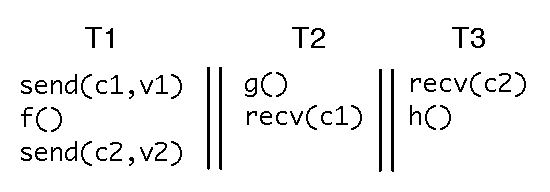
\includegraphics{Figures/IntroCode1}
\end{center}

\noindent Thread T1 performs a synchronous send on channel \cf{c1} that is
received by thread T2, after it computes \cf{g()}.  After the communication is
performed, T1 evaluates \cf{f()}, and then sends \cf{v2} on channel \cf{c2},
which is received by thread T3.  Upon receipt, T3 evaluates \cf{h()}. Assuming
\cf{f},\cf{g}, and \cf{h} perform no communication action of their own, the
synchronous communication on \cf{c1} by T1 could have been safely converted
into an asynchronous action in which \cf{v1} is buffered, and read by T2 later
upon evaluation of \cf{g()}.  The observable behavior of the program in both
cases (i.e., treating the initial send synchronously or asynchronously) would
be the same.

\begin{figure}[b]
\centering
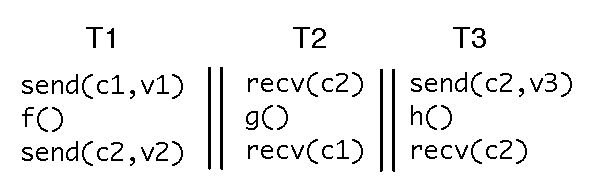
\includegraphics{Figures/IntroCode2}
\caption{Performing the first \cf{send} in T1 asynchronously is not meaning
preserving with respect to synchronous evaluation.}
\label{fig:intro2}
\end{figure}

Unfortunately, na\"{i}vely replacing synchronous communication with an
asynchronous one is not usually meaning-preserving as the example in
Figure~\ref{fig:intro2} illustrates. Under a synchronous evaluation protocol,
T2 would necessarily communicate first with T3, receiving \cf{v3} on channel
\cf{c2}.  It is then able to receive \cf{v1} from T1; finally, T1 can
communicate \cf{v2} to T3.  If the \cf{send(c1,v1)} operation by T1 were
replaced by \cf{asend(c1,v1)}, the first receive on T2 has, in addition to the
first send on T3, a \emph{new potential matching opportunity} -- the send of
\cf{v2} on channel \cf{c2}. If the receive by T2 matches with the send of
\cf{v2} on channel \cf{c2}, it is impossible to satisfy the send on T3. Thus,
this asynchronous execution exhibits a new behavior not possible using just
synchronous operators.

The distinction between these two executions can be explained in terms of a
dependence graph that captures both intra- and inter-thread data- and
control-flow.  We can depict the executions by explicitly drawing these
dependencies as shown below:

\begin{center}
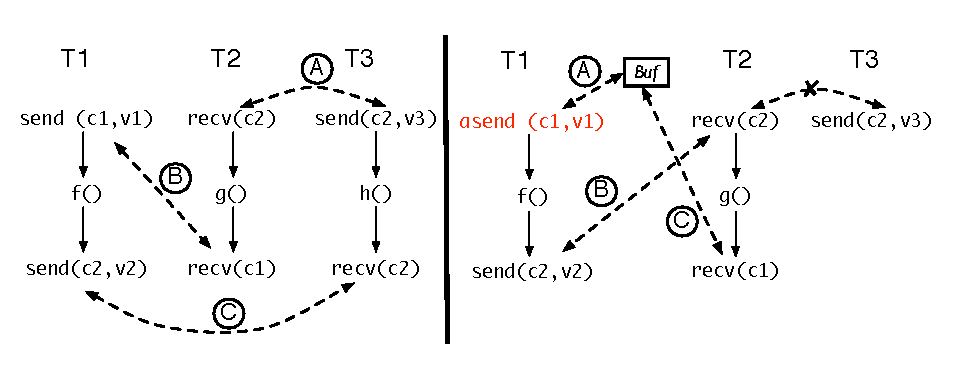
\includegraphics{Figures/IntroDepGraph}
\end{center}

\noindent The dashed edges reflect communication and synchronization
dependencies among threads, while solid edges capture thread-local
control-flow. A bi-directional edge connects a sender with either a
receiver, in the case of a synchronous send, or a buffer, in the case where
it is asynchronous.  In both instances, there is a synchronization
dependence between endpoints, and a data dependence from the sender to
either the matching receiver or buffer.  The left-hand side of the figure
shows a possible execution in which all operations are synchronous; the
right considers an execution in which the initial send by T1 is
asynchronous.  The labels on the edges reflect the order in which
communication actions are executed.

\newcommand*\mycirc[1]{%
  \begin{tikzpicture}[baseline=(char.base)]
    \node[shape=circle,draw,inner sep=.3pt] (char) {#1};
  \end{tikzpicture}}

The synchronous execution on the left reflects the description given earlier.
The asynchronous execution on the right depicts the send on thread T1 buffering
its data (\mycirc{A}), thus allowing the synchronous communication between T1
and T2 (\mycirc{B}); this action prohibits communication between T2 and T3.  T2
subsequently receives \cf{v1} from the buffer associated with channel \cf{c1}
(\mycirc{C}).  This behavior could not be realized by any synchronous
execution: \mycirc{B} could never have been performed if the send operation on
channel \cf{c1} was not asynchronous.

The formalization of \emph{well-formed executions}, those that are the result
of asynchronous evaluation of CML send operations, but which nonetheless are
observably equivalent to a synchronous execution, and the means by which
erroneous executions, such as the right-hand execution above, can be detected
and repaired, form the focus of this chapter. Specifically, we make the
following contributions:

\begin{itemize}

\item We present the rationale for a \emph{relaxed execution model} for CML
that specifies the conditions under which a synchronous operation can be safely
executed asynchronously.  Our model allows applications to program with the
simplicity and composability of CML synchronous events, but reap the
performance benefits of implementing communication asynchronously.

\item We develop an axiomatic formulation of the model that can be used to
reason about correctness in terms of causal dependencies captured by a
\emph{happens-before} relation.  We relate this definition to an operational
semantics that specifies relaxed execution behavior for communicating actions,
and relate the set of traces admitted by the operational semantics to the safe
executions defined by the axiomatic formulation.

\item A distributed implementation, \rxcml, that treats asynchronous
communication as a form of \emph{speculation} is described. A mis-speculation,
namely the execution that could not have been realized using only synchronous
communication, is detected using a runtime instantiation of our axiomatic
formulation. An un-coordinated, distributed checkpointing mechanism is utilized
to rollback and re-execute the offending execution synchronously, which is
known to be safe.

\item Several case studies on a realistic cloud deployment demonstrate the
utility of the model in improving the performance of CML programs in
distributed environments without requiring \emph{any} restructuring of
application logic to deal with asynchrony.

\end{itemize}

\section{Motivation}

To motivate the utility of safe relaxation of synchronous behavior, consider
the problem of building a distributed chat application. The application
consists of a number of participants, each of whom can broadcast a message to
every other member in the group. The invariant that must be observed is that
any two messages sent by a participant must appear in the same order to all
members. Moreover, any message \cf{Y} broadcast in response to a previously
received message \cf{X} must always appear after message \cf{X} to every
member. Here, message \cf{Y} is said to be \emph{causally dependent} on
message \cf{X}.

\begin{figure}
\begin{lstlisting}
datatype 'a bchan = BCHAN of ('a chan list (*val*) *
															unit chan list (*ack*))

(* Create a new broadcast channel *)
fun newBChan (n: int) (* n = number of participants *) =
  BCHAN(tabulate(n,fn _ => channel()), tabulate(n,fn _ => channel()))

(* Broadcast send operation *)
fun bsend (BCHAN (vcList, acList), v: 'a, id: int) : unit =
let
	val _ = map (fn vc => if (vc = nth (vcList, id)) then ()
												else send (vc, v))
						vcList (* phase 1 -- Value distribution *)
	val _ = map (fn ac => if (ac = nth (acList, id)) then ()
												else recv ac)
						acList (* phase 2 -- Acknowledgments *)
in ()
end

(* Broadcast receive operation *)
fun brecv (BCHAN (vcList, acList), id: int) : 'a=
let val v = recv (nth (vcList, id))
		val _ = send (nth (acList, id), ())
in v
end
\end{lstlisting}
\caption{Synchronous broadcast channel}
\label{code:bchan}
\end{figure}

Building such an application using a centralized server is straightforward, but
hinders scalability. In the absence of central mediation, a causal broadcast
protocol~\cite{Birman87} is required. One possible encoding of causal broadcast
using CML primitives is shown in Figure~\ref{code:bchan}. A broadcast operation
involves two phases.  In the first phase, values (i.e., messages) are
synchronously communicated to all receivers (except to the sender).  In the
second phase, the sender simulates a barrier by synchronously receiving
acknowledgments from all recipients.

The synchronous nature of the broadcast protocol along with the fact that the
acknowledgment phase occurs only after message distribution ensure that no
member can proceed immediately after receiving a message until all other
members have also received the message. This achieves the desired causal
ordering between broadcast messages since every member would have received a
message before the subsequent causally ordered message is generated. We can
build a distributed group chat server using the broadcast channel as shown
below.

\lstset{numbers=none}
\begin{lstlisting}
(* bc is broadcast chan, daemon is spawn as a separate thread *)
fun daemon id = display (brecv (bc, id)); daemon id
fun newMessage (m, id) = display m; bsend (bc, m, id)
\end{lstlisting}
\lstset{numbers=left,numberstyle=\tiny,stepnumber=1}

Assume that there are $n$ participants in the group, each with a unique
identifier \emph{id} between $0$ and $n-1$. Each participant runs a local
\emph{daemon} thread that waits for incoming messages on the broadcast channel
\cf{bc}. On a reception of a message, the daemon displays the message and
continues waiting. The clients broadcast a message using \cf{newMessage} after
displaying the message locally.  Observe that remote messages are only
displayed after all other participants have also received the message. In a
geo-distributed environment, where the communication latency is very high, this
protocol results in a poor user experience that degrades as the number of
participants increases.

Without making wholesale (ideally, zero!) changes to this relatively simple
protocol implementation, we would like to improve responsiveness, while
preserving correctness.  One obvious way of reducing latency overheads is to
convert the synchronous sends in {\tt bsend} to an asynchronous variant that
buffers the message, but does not synchronize with a matching receiver. There
are two opportunities where asynchrony could be introduced, either during value
distribution or during acknowledgment reception. Unfortunately, injecting
asynchrony at either point is not guaranteed to preserve causal ordering on the
semantics of the program.

\begin{figure}
\begin{centering}
	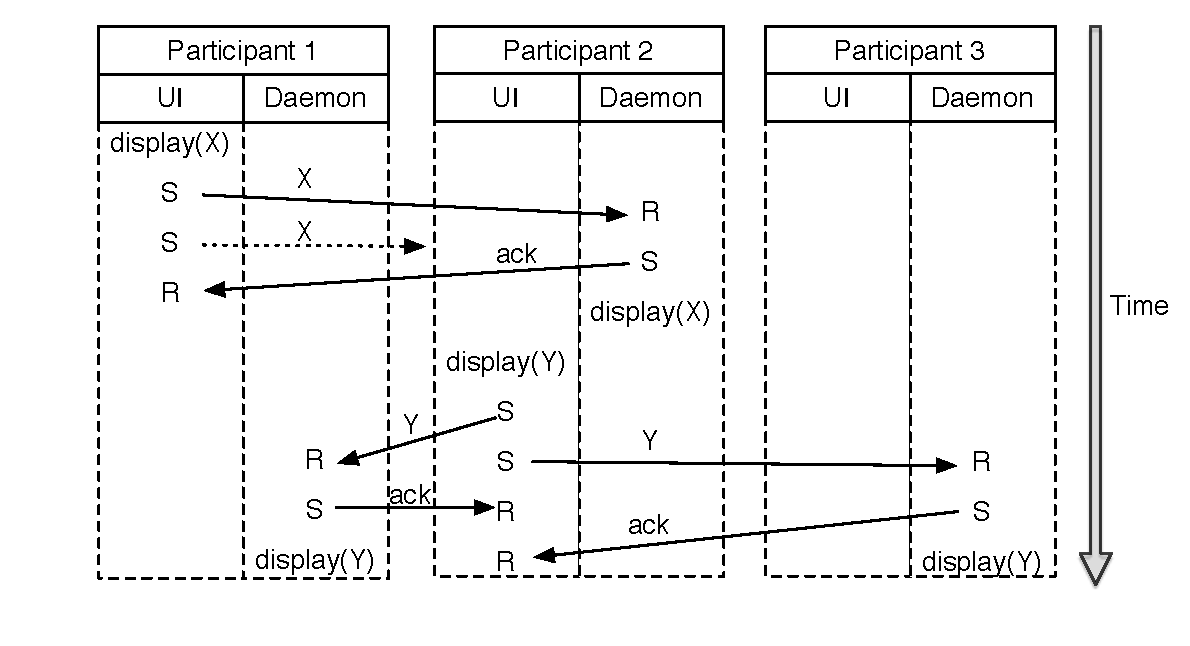
\includegraphics[width=\textwidth] {Figures/ChatServer_AsyncValue}
	\caption{Incorrect execution due to unsafe relaxation of sends during
	broadcast. Dotted arrow represents in-flight message.}
	\label{fig:CS_asend_value}
\end{centering}
\end{figure}

Consider the case where the value is distributed asynchronously. Assume that
there are three participants: $p_1$, $p_2$, and $p_3$. Participant $p_1$ first
types message \cf{X}, which is seen by $p_2$, who in turn types the message
\cf{Y} after sending an acknowledgment. Since there is a causal order between
the message {\codecf X} and {\codecf Y}, $p_3$ must see {\codecf X} followed by
{\codecf Y}. Figure~\ref{fig:CS_asend_value} shows an execution where this is
not the case. In the figure, uninteresting messages have been elided for
clarity. The key observation is that, due to asynchrony, message \cf{X} sent
by the $p_1$ to $p_3$ might be \emph{in-flight}, while the causally dependent
message \cf{Y} sent by $p_2$ reaches $p_3$ out-of-order. This leads to a
violation of the protocol's invariants.

Similarly, it is easy to see that sending acknowledgments message
asynchronously is also incorrect. This would allow a participant that receives
a message to asynchronously send an acknowledgment, and proceed before all
other participants have received the same message. As a result, causal
dependence between messages is lost.

To quantify these issues in a realistic setting, we implemented a group chat
simulator application using a distributed extension of the MultiMLton Standard
ML compiler. We launched three Amazon EC2 instances, each simulating a
participant in the group chat application, with the same communication pattern
described in the discussion above. In order to capture the geo-distributed
nature of the application, participants were placed in three different
availability zones -- EU West (Ireland), US West (Oregon), and Asia Pacific
(Tokyo), resp.

During each run, $p_1$ broadcasts a message \cf{X}, followed by $p_2$
broadcasting \cf{Y}. We consider the run to be successful if the participant
$p_3$ sees the messages \cf{X},\cf{Y}, in that order.  The experiment was
repeated for 1K iterations. We record the time between protocol initiation and
the time at which each participant gets the message \cf{Y}. We consider the
largest of the times across the participants to be the running time. The
results are presented below.

\begin{center}
\begin{tabular}{ | l | r | r |}
	\hline
	\emph{Execution} 					& \emph{Avg.time (ms)} & \emph{Errors} \\
  \hline
	\emph{Sync}								& 1540	\ci{53} &	0 \ci{0} \\
	\emph{Unsafe Async} 			& 520		\ci{17} & 7 \ci{2} \\
	\emph{Safe Async (\rxcml)}	& 533		\ci{13} & 0 \ci{0} \\
  \hline
\end{tabular}
\end{center}

The \emph{Unsafe Async} row describes the variant where both value and
acknowledgment distribution is performed asynchronously; it is three times as
fast as the synchronous variant.  However, over the total set of 1K runs, it
produced seven erroneous executions. The \emph{Safe Async} row illustrates our
implementation, \rxcml, that detects erroneous executions on-the-fly and
remediates them. The results indicate that the cost of ensuring safe
asynchronous executions is quite low for this application, incurring only
roughly 2.5\% overhead above the unsafe version. Thus, in this application, we
can gain the performance benefits and responsiveness of the asynchronous
version, while retaining the simplicity of reasoning about program behavior
synchronously.

\section{Axiomatic Semantics}
\label{sec:axiomatic}

We introduce an axiomatic formalization for reasoning about the relaxed
behaviors of a concurrent message-passing programs with dynamic thread
creation. Not surprisingly, our formulation is similar in structure to
axiomatic formalizations used to describe, for example, relaxed memory
models~\cite{BMM,Sarkar09,Sewell10}.

An \emph{axiomatic execution} is captured by a set of \emph{actions} performed
by each thread and the relationship between them. These actions abstract the
relevant behaviors possible in a CML execution, relaxed or otherwise. Relation
between the actions as a result of sequential execution, communication, thread
creation and thread joins define the dependencies that any sensible execution must
respect. A relaxed execution, as a result of speculation, admits more behaviors
than observable under synchronous CML execution. Therefore, to understand the
validity of executions, we define a \emph{well-formedness} condition that
imposes additional constraints on executions to ensure their observable effects
correspond to correct CML behavior.

We assume a set of $\ThreadClass$ threads, $\ChannelClass$ channels, and
$\ValueClass$ values.  The set of actions is provided below. Superscripts $m$
and $n$ denote a unique identifier for the action.

\begin{mathpar}
\begin{array}{rcll}
\R{Actions} \; \ActionClass{}
	& \coloneqq & b_t 			& \R{(t starts)} \\
	& \mid      & e_t 			& \R{(t ends)} \\
	& \mid      & j_t^mt' 	& \R{(t detects t' has terminated)} \\
	& \mid      & f^m_tt' 	& \R{(t forks a new t')} \\
	& \mid 	    & s_t^mc,v 	& \R{(t sends value v on c)} \\
	& \mid      & r_t^mc   	& \R{(t receives a value v on c)} \\
	& \mid 	    & p_t^mv	 	& \R{(t outputs an observable value v)}
\end{array}

c      ~ \in ~ \ChannelClass ~ \R{(Channels)} \tab
t,t'   ~ \in ~ \ThreadClass ~ \R{(Threads)} \tab
v     ~ \in ~ \ValueClass ~ \R{(Values)} \tab
m,n ~ \in ~ \NumberClass ~ \R{(Numbers)}
\end{mathpar}

\noindent Action $b_t$ signals the initiation of a new thread with identifier
$t$; action $e_t$ indicates that thread $t$ has terminated.  A join action,
$j_t^mt'$, defines an action that recognizes the point where thread $t$ detects
that another thread $t'$ has completed.  A thread creation action, where thread
$t$ spawns a thread $t'$, is given by $f^m_tt'$. Action $s_t^mc,v$ denotes the
communication of data $v$ on channel $c$ by thread $t$, and $r_t^mc$ denotes
the receipt of data from channel $c$.  An external action (e.g., printing) that
emits value $v$ is denoted as $p_t^mv$.  We can generalize these individuals
actions into a family of related actions:
\begin{mathpar}
\begin{array}{lcll}
\ActionClass{r} &=& \{r_t^mc \mid t \in\ThreadClass\} & \R{(Receives)} \\
\ActionClass{s} &=& \{s_t^mc,v \mid t \in\ThreadClass, v\in\ValueClass\} & \R{(Sends)} \\
\ActionClass{c} &=& \ActionClass{s} \cup \ActionClass{r} & \R{(Communication)} \\
\ActionClass{o} &=& \{p_t^mv		 \mid	t \in\ThreadClass,v\in\ValueClass\} & \R{(Observables)} \\
\end{array}
\end{mathpar}

\noindent {\bf Notation.} We write $T(\alpha)$ to indicate the thread in which
action $\alpha$ occurs, and write $\,V(s_t^mc,v)$ to extract the value $v$
communicated by a send action. Given a set of actions $\ActionSet \in
2^\ActionClass{}$, $\ActionSet_x = \ActionSet \cap \ActionClass{x}$, where
$\ActionClass{x}$ represents one of the action classes defined above.

\begin{definition}[Axiomatic Execution]
An axiomatic execution is defined by the tuple $\E \coloneqq \Exec$ where:
\begin{itemize}
\item $\program$ is a program.
\item $\ActionSet$ is a set of actions.
\item $\po \; \subseteq \ActionSet \times \ActionSet$ is the program order,
  a disjoint union of the sequential actions of each thread (which is a
  total order).
\item $\co \; \subseteq (\ActionSet_s \times \ActionSet_r) \cup (\ActionSet_r
	\times \ActionSet_s)$ is the communication order which is a symmetric
	relation established between matching communication actions (i.e., $\alpha
	\co \beta \implies \beta \co \alpha$). Moreover, a send and its matching
	receive must operate over the same channel (i.e., $s_t^mc,v \co r_{t'}^n{c'}
	\implies c = c'$).
\end{itemize}
\label{defn:exec}
\end{definition}

Additionally, there is an obvious ordering on thread creation and execution, as
well as the visibility of thread termination by other threads:

\begin{definition}[Thread Dependence]
\label{def:thr_dep}
If $\alpha = f_t^mt'$ and $\beta = b_{t'}$ or  $\alpha = e_t$ and $\beta = j_{t'}^mt$
then $\alpha \td \beta$ holds.
\end{definition}


\begin{definition}[Happens-before relation]
\label{def:hb}
The \textit{happens-before} order of an execution is the transitive closure of
the union of program order, thread dependence order, and actions related by
communication and program order:
\begin{mathpar}
\begin{array}{lll}
\hb & = & (\po \cup \td \cup \\
    &   &  \{ (\alpha,\beta)\ |\ \alpha \co \alpha' \wedge \alpha' \po \beta \}\ \cup \\
    &   &  \{ (\beta,\alpha)\ |\ \beta \po \alpha' \wedge \alpha' \co \alpha \})^+
\end{array}
\end{mathpar}
\end{definition}

\noindent For any two actions $\alpha,\beta \in \ActionSet$, if $\alpha \nbihb
\beta$, then $\alpha$ and $\beta$ are said to be \textit{concurrent} actions.
Importantly, our happens-before relation defines a preorder. A preorder is a
reflexive transitive binary relation. Unlike partial orders, preorders are not
necessarily anti-symmetric, i.e. they may contain cycles.

\begin{definition}[Happens-before Cycle]
A cycle exists in a happens-before relation if for any two actions
$\alpha, \beta$ and $\alpha \hb \beta \hb \alpha$.
\end{definition}

\lstset{numbers=none}
\begin{figure}
\begin{lstlisting}
(* current thread is t1 *)
val t2 = spawn (fn () => recv c2; print "2"; recv c1)

val t3 = spawn (fn () => send(c2,v2); print "3"; recv c2)

val _ = send(c1,v1)
val _ = print "1"
val _ = send(c2,v2)
\end{lstlisting}
\caption{A CML Program with potential for mis-speculation.}
\label{code:simple}
\end{figure}
\lstset{numbers=left,numberstyle=\tiny,stepnumber=1,frame=single}

\begin{figure}
\begin{minipage}{0.5\textwidth}
\subfigure[Well-formed execution]{\label{fig:well}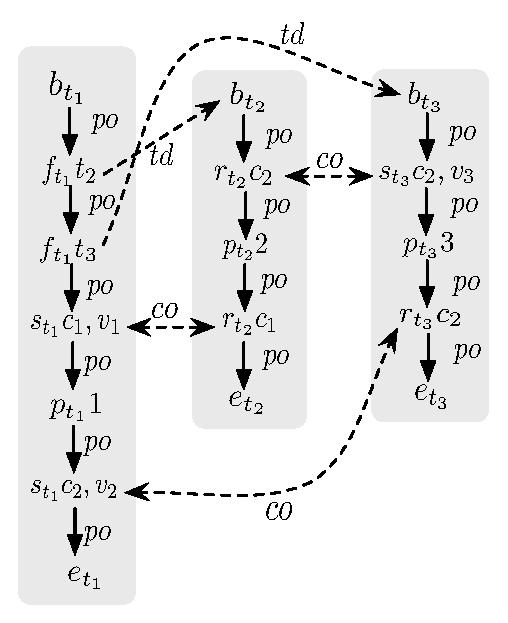
\includegraphics[width=1\textwidth]{Figures/AxiomaticExecution}}
\end{minipage}
\hfill
\begin{minipage}{0.5\textwidth}
\subfigure[Ill-formed execution]{\label{fig:ill}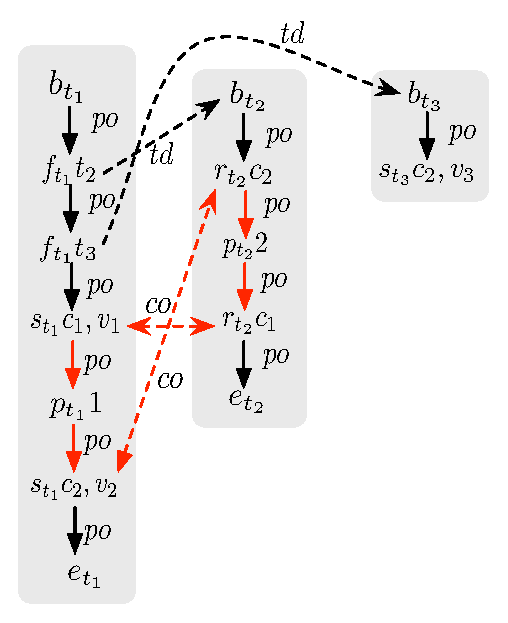
\includegraphics[width=1\textwidth]{Figures/AxiomaticExecution-1}}
\end{minipage}
\caption{Potential axiomatic executions of the CML program presented in Figure~\ref{code:simple}.}
\label{fig:pgm_and_execs}
\end{figure}

We provide an example to illustrate these definitions and to gain an insight
into erroneous executions that manifest as a result of speculative
communication. Consider the simple CML program (Figure~\ref{code:simple}) which
shows a simple CML program and two possible executions
(Figure~\ref{fig:pgm_and_execs}). The execution in Figure~\ref{fig:well}
imposes no causal dependence between the observable actions (i.e., print
statements) in $t_2$ or $t_3$; thus, an interleaving derived from this
execution may permute the order in which these statements execute. All
interleavings derivable from this execution correspond to valid CML behavior.

In contrast, the execution depicted in Figure~\ref{fig:ill}, exhibits a
happens-before cycle between $t_1$ and $t_2$, through a combination of program
and communication order edges. \emph{Such cyclic dependences never manifest in
any correct CML execution}. Cyclic dependences may however manifest when
synchronous sends are speculatively discharged asynchronously. We must
therefore strengthen our notion of correct executions to discard those that
contain such cycles.

To do so, we first note that the semantics as currently presented is concerned
only with actions that introduce some form of causal dependence either within a
thread (via program order) or across threads (via thread dependence or
communication order). However, a real program also does computation, and
reasoning about an execution's correctness will require us to specify these
actions as well. To facilitate this reasoning, we abstract the intra-thread
semantics, and parameterize our definition of an axiomatic execution accordingly.

\subsubsection{Intra-thread semantics} The intra-thread semantics is abstracted
in our formulation via a labeled transition system.  Let $\intrastate$ denote
the intra-thread state of a thread; its specific structure is not interesting
for the purposes of the axiomatic definition. A labeled transition between
intra-thread states is captured by the relation, $\intratrans{.} \subseteq
\intrastate \times \intralabel \times \intrastate$, given to each thread $t \in
\ThreadClass$. The transition labels are in the set $\intralabel =
(\ActionClass{} \setminus \ActionClass{r}) \cup (\ActionClass{r} \times
\ValueClass) \cup \{\tau\}$.  Thus, a thread can either take a global action
step (e.g., creating another thread, performing a send action, ending a thread,
etc.), execute a \emph{silent} thread-local computation (denoted by label
$\tau$), or execute a receive action that receives the value associated with
the label. The requirements on the intra-thread semantics are:

\begin{itemize}
\item $\intratrans{.}$ can only relate states belonging to the same thread.
\item there is an initial state \ready: no transition leads to it,
	and a thread $t$ steps from it if and only if it emits a begin action $b_t$.
\item there is a final state \done: a thread leads to it if and only if it
	emits an end action $e_t$ and no transition leads from it.
\end{itemize}

\begin{definition}[Intra-trace]
\label{def:intra-trace}
Let $tr = \bar{\alpha}$ be a sequence of actions in set $\ActionSet$, and
$\co$ be a communication order on $\ActionSet$. Given a thread
$t \in \ThreadClass$ in a program $\program$, $tr$ is a valid intra-trace for
$t$ if there exists a set of states $\{\delta_0, \delta_1, \ldots \}$, and a
set of labels $\bar{l} = \{l_0, l_1,\ldots\}$ such that:
%
\begin{itemize}
\item for all $\alpha_i \in \bar{\alpha}, T(a) = t$
\item $\delta_0$ is the initial state \ready
\item for all $0 \leq i, \delta_{i} \intratrans{l_i} \delta_{i+1}$
\item the projection $\bar{\beta}$ of $\bar{l}$ to non-silent labels is such
	that $\beta_i = (\alpha_i, V(\gamma_i))$ if $\alpha_i \in \ActionSet_r$ and
	$\alpha_i \co \gamma_i$, or $\beta_i = \alpha_i$ otherwise.

\end{itemize}
\end{definition}

\noindent We write $\intraTraceSet[t]$ set of such pairs $(tr,\co)$ for
$\program$.

\begin{definition}[Well-formed Execution]
\label{def:well-formed}
An execution $E \coloneqq \Exec$ is well-formed if the following
conditions hold:
%
\begin{enumerate}
\item Intra-thread consistency: for all threads $t \in \ThreadClass,
	\;(\restrict{\po}{t}, \co) \in \intraTraceSet[t]$
\item Happens-before correctness: The happens-before relation $\hb$ constructed
	from $E$ has no cycles.
\item Observable correctness: Given $\alpha  \in \ActionSet_{o}$ and  $\beta
	\in \ActionSet_{c}$ if $\beta \hb \alpha$ then there exists $\beta' \in
	\ActionSet_{c}$ s.t. $\beta \co \beta'$.
\end{enumerate}
\end{definition}

For an axiomatic execution $\E \coloneqq \Exec$ to be well-formed, the actions,
program order and communication order relations must have been obtained from a
valid execution of the program $\program$ as given by the intra-thread
semantics defined above (1). As we noted in our discussion of
Figure~\ref{fig:pgm_and_execs}, no valid execution of a CML program may involve
a cyclic dependence between actions; such dependencies can only occur because
of \emph{speculatively} performing what is presumed to be a synchronous send
operation (2).

Finally, although the relaxed execution might speculate, i.e., have a send
operation transparently execute asynchronously, the observable behavior of such
an execution should mirror some valid non-speculative execution, i.e., an
execution in which the send action was, in fact, performed synchronously.  We
limit the scope of speculative actions by requiring that they complete (i.e.,
have a matching recipient) before an observable action is performed (3).
Conversely, this allows communication actions not preceding an observable
action to be speculated upon. Concretely, a send not preceding an externally
visible action can be discharged asynchronously. The match and validity of the
send needs to be checked only before discharging the next such action. This is
the key idea behind our speculative execution framework.

\subsubsection{Safety.} An axiomatic execution represents a set
of interleavings, each interleaving defining a specific total order that is
consistent with the partial order defined by the execution\footnote{Two
ordering relations $P$ and $Q$ are said to be \textit{consistent} if
$\forall x,y, \neg(xPy \conj yQx)$.}.  The well-formedness conditions of an
axiomatic execution implies that any observable behavior of an interleaving
induced from it must correspond to a synchronous CML execution. The
following two definitions formalize this intuition.

\begin{definition}[Observable dependencies]
\label{def:od}
In a well-formed axiomatic execution $\E \coloneqq \Exec$, the observable
dependencies $\ActionSet_{od}$ is the set of actions that precedes (under
$\hb$) some observable action, i.e., $\ActionSet_{od} = \{\alpha \ALT \alpha \in
\ActionSet, \beta \in \ActionSet_{o}, \alpha \hb \beta\}$.
\end{definition}

\begin{definition}[$\cml$ Execution]
\label{def:cml}
Given a well-formed axiomatic execution $\E \coloneqq \Exec$, the pair $(\E,
\toto)$ is said to be in $\cml(\program)$ if $\toto$ is a total order on
$\ActionSet_{od}$ and $\toto$ is consistent with $\hb$.
\end{definition}

In the above definition, an interleaving represented by $\toto$ is only possible
since the axiomatic execution is well-formed, and thereby does not contain a
happens-before cycle.

\begin{lemma}
\label{lem:toto_hb}
If a total order $\toto$ is consistent with $\hb$, then $\hb$ does not contain
a cycle involving actions in $\ActionSet_{od}$.
\end{lemma}

%% \begin{proof}
%% Assume $\alpha \hb \beta \hb \alpha$, then either $\alpha \toto \beta$ or
%% $\beta \toto \alpha$. If $\alpha \toto \beta$, then pick $\beta \hb \alpha$ and
%% show that $\toto$ is not consistent with $\hb$. Similarly for the other case.
%% \end{proof}

Next, we show that a well-formed axiomatic execution respects the safety
property of non-speculative execution of a CML program. When a CML program
evaluates non-speculatively, a thread performing a communication action is
blocked until a matching communication action is available. Hence, if
$(\Exec,\toto) \in \cml(\program)$, and a communication action $\alpha$ on a
thread $t$ is followed by an action $\beta$ on the same thread, then it must be
the case that there is a matching action $\alpha \co \alpha'$ that
happened before $\beta$ in $\toto$. This is captured in the following theorem.

\begin{theorem}
Given a CML execution $(\E, \toto) \in \cml(\program)$, $\forall \alpha,\beta$
such that $\alpha \in \ActionClass{c}, T(\alpha) = T(\beta), \alpha \toto \beta$,
there exists an action $\alpha \co \alpha'$ such that $\alpha' \toto
\beta$.
\end{theorem}
\begin{proof}
Let $\E \coloneqq \Exec$. First, we show that $\alpha' \in \ActionSet$. Since
$\alpha \toto \beta$, $\alpha \in \ActionSet_{od}$, by
Definition~\ref{def:cml}. By Definition~\ref{def:od}, there exists some $\gamma
\in \ActionSet_o$ such that $\alpha \hb \gamma$. Since $\E$ is well-formed and
$\alpha \hb \gamma$, by Definition~\ref{def:well-formed}, there exists an
$\alpha' \in \ActionSet$ such that $\alpha \co \alpha'$.

Next, we show that $\alpha' \in \ActionSet_{od}$. By Definition~\ref{def:hb},
$\alpha' \co \alpha \hb \gamma$ implies $\alpha' \hb \gamma$. Hence, $\alpha'
\in \ActionSet_{od}$, and is related by $\toto$. Finally, since $T(\alpha) =
T(\beta)$ and $\alpha \toto \beta$, $\alpha \po \beta$. And, $\alpha' \co
\alpha \po \beta$ implies $\alpha' \hb \beta$. By Lemma~\ref{lem:toto_hb} and
Definition~\ref{def:cml}, $\alpha' \toto \beta$.
\end{proof}

\section{Operational Semantics}

\begin{figure}
\begin{minipage}[t]{\columnwidth}
\begin{smathpar}
\begin{array}{lclcl}
e & \in & {\tt Exp} & := 		& v \ALT x \ALT e \; e \ALT \chan() \ALT \print(e) \ALT \spawn(e) \\
	&			&						& \ALT 	&	\send(e,e) \ALT 	\recv(e) \ALT \join(e)\\
v & \in & {\tt Val} & := 		& \unit \ALT c \ALT \lambda\,x.e \ALT t \\
\end{array}
\end{smathpar}
\end{minipage}
%
\begin{minipage}[t]{\columnwidth}
\begin{smathpar}
\begin{array}{lcl}
E & := 		& \bullet \ALT E\;e \ALT v\;E \ALT \print(E) \\
  & \ALT 	& \spawn(E) \ALT \send(E,e) \ALT \send(c,E) \\
	& \ALT	& \recv(E) \ALT \join(E)
\end{array}
\end{smathpar}
\end{minipage}

\begin{minipage}[t]{\columnwidth}
\begin{smathpar}
\begin{array}{lclcl}
c & \in & {\tt ChannelId}\\
\alpha,\beta 	& \in & {\tt Action} & := & \ActionClass\ \ALT (\alpha,\beta) \ALT\ \tau_t \ALT \commit{\program}{\trace}\\
\ActionSoup 	& \in & {\tt SendSoup}		& := & \ActionClass{s}\\
\localstate 	& \in & {\tt LocalState} & := & e \ALT \readyOp{e} \ALT \doneOp \\
t 						& \in & {\tt ThreadId}\\
\thread 			& \in & {\tt Thread} 				& := & (t,\localstate) \\
\threadsoup 	& \in & {\tt ThreadSoup}		& := & \emptyset \ALT \thread \;\|\; \threadsoup\\
\langle \threadsoup,\ActionSoup \rangle	& \in & \ProgramState
\end{array}
\end{smathpar}
\end{minipage}
\caption{Syntax and states for the relaxed execution semantics of a subset of CML.}
\label{sem:rxcml_op_syntax}
\end{figure}

\begin{figure}
\begin{smathpar}
\begin{array}{cl}

\RULE
{\\ }
{\PrgState{(\lambda\,x.e) v}{\ActionSoup}
\intertrans{\tau_t}
\PrgState{e[x/v]}{\ActionSoup}} & \rulelabel{App} \\ \\

\RULE
{c \;\; \fresh \;\;\; }
{\PrgState{\chan()}{\ActionSoup}
\intertrans{\tau_t}
\PrgState{c}{\ActionSoup}} & \rulelabel{Chan} \\ \\

\RULE
{\\
}
{\langle (t,\readyOp{e}) \;\|\; \threadsoup, \ActionSoup \rangle
 \intertrans{b_t}
 \langle (t,e) \;\|\; \threadsoup, \ActionSoup \rangle} & \rulelabel{Begin} \\ \\

\RULE
{}
{\langle (t,v) \;\|\; \threadsoup,\ActionSoup \rangle
 \intertrans{e_t}
 \langle (t,\doneOp) \;\|\; \threadsoup, \ActionSoup \rangle} & \rulelabel{End} \\ \\

\RULE
{}
{\PrgState{\spawn\,e}{\ActionSoup}
\intertrans{f_t^it'}
\langle (t,\opIntraState{t'}) \;\|\; (t',\readyOp{e}) \;\|\; \threadsoup, \ActionSoup \rangle} & \rulelabel{Spawn} \\ \\

\RULE
{}
{\langle (t,\opIntraState{\join\,t'}) \;\|\; (t',\doneOp) \;\|\; \threadsoup, \ActionSoup \rangle
 \intertrans{j_t^it'}
 \langle (t,\opIntraState{\unit}) \;\|\; (t',\doneOp) \;\|\; \threadsoup, \ActionSoup \rangle} & \rulelabel{Join} \\ \\

\RULE
{\\}
{\PrgState{\print\,v}{\ActionSoup} \intertrans{p_t^iv}
\PrgState{\unit}{\ActionSoup}} & \rulelabel{Print} \\ \\

\RULE
{\alpha = s_t^ic,v}
{\PrgState{\send(c,v)}{\ActionSoup}
 \intertrans{\alpha}
 \PrgState{\unit}{\ActionSoup \cup \{\alpha\}}} & \rulelabel{Send} \\ \\

\RULE
{\alpha = r_t^ic \;\;\; \beta = (s_{t'}^jc,v) \in \ActionSoup}
{\PrgState{\recv\,c}{\ActionSoup}
\intertrans{(\alpha,\beta)}
\PrgState{v}{\ActionSoup \setminus \beta}} & \rulelabel{Recv} \\ \\

\RULE
{\wf{(\program,\trace)}}
{\langle\threadsoup,\ActionSoup\rangle
\intertrans{\commit{\program}{\trace}}
\langle\threadsoup,\ActionSoup\rangle} & \rulelabel{Commit}

\end{array}
\end{smathpar}
\caption{A relaxed execution operational semantics for a subset of CML.}
\label{fig:op_semantics}
\end{figure}

The axiomatic semantics provides a declarative way of reasoning about
executions. However, it is unclear how to use this semantics to
\emph{execute} a CML program that performs the sends asynchronously
while ensuring that the observable behaviors correspond to a
synchronous execution of the program; that is, how we can we ensure
that implementations produce relaxed executions that always conform to
a CML execution in the sense of Definition~\ref{def:cml}?  In this
section, we present an operational definition of a relaxed execution
as a labeled transition system that allows us to express the
constraints necessary to prevent non-CML observable behaviors.

The operational machine, $\rel$, takes as its input an operational execution,
which is composed of a program, and a trace $\trace$ of \emph{operational
actions}. It evaluates the program according to the trace, by manipulating a
\emph{send soup}, an unordered set into which pending sends are added
asynchronously.  Informally, we can think of the trace as a history or log of
actions we wish to perform; the machine either accepts the trace, if executing
the actions found in the trace using the reduction rules leads to a CML
execution (as defined by Definition~\ref{def:cml}), or gets stuck otherwise. An
operational action $\alpha \in \ActionClass{op}$ is either:

\begin{itemize}

\item an action in $\ActionClass{} \setminus \ActionClass{r}$.
\item a pair in $\ActionClass{r} \times \ActionClass{s}$ where each receive
	action is paired up with the matching send action on the same channel,
\item a \emph{silent} action $\tau_t$ indexed by a thread identifier that
  indicates the evaluation of a computation step (e.g., a function call).
\item a \emph{commit} action $\commit{\program}{\trace}$ that checks whether
  the machine state is well-formed in the sense of
  Definition~\ref{def:well-formed}.  Intuitively, a well-formed machine
  state is one that could have been reached if all \cf{send} operations
  were executed synchronously.

\end{itemize}

\begin{definition}[Operational Execution]
An operational execution is a pair $(\program,tr)$, where $\program$ is a
program and $tr \in \bar{\ActionClass{op}}$, and there are no duplicates in
$tr$.
\end{definition}

The semantics used to interpret the trace is given in
Figure~\ref{fig:op_semantics}.  The program state is composed of a tuple
with $\threadsoup$ representing the pool of concurrently executing threads
and a collection of unmatched send actions $\ActionSoup$. Each thread in
$\threadsoup$ is a tuple with a thread id and a local state.  This state is
either an initial state $\readyOp{e}$ containing the expression that will
be evaluated by this thread, or a completed state $\doneOp$, or the
expression being evaluated by this thread.  Each state transition is affixed
with an action drawn from the trace that is used by the machine to determine
which rule to apply, as we describe below.

The source language contains function abstraction, application, first-class
channels, a thread creation operation ({\sf spawn}), message-passing
primitives on these channels, and a {\sf print} statement to capture an
observable action.  Reductions are labeled with operational actions. Rules
{\sc App} and {\sc Chan} represent silent (thread-local) actions.  The {\sc
  Spawn} rule creates a new thread with the initial local state
$\readyOp{e}$. Rule {\sc Begin} initiates execution of the thread from its
initial state.  A thread moves to the $\doneOp$ local state once the
expression being evaluated is reduced to a value (Rule {\sc End}). The
completed thread remains in the thread pool so that other threads may also
join on it.  A thread can wait on another thread's completion by joining on
its thread identifier. The calling thread is paused until the joined thread
moves to the final local state $\doneOp$ (Rule {\sc Join}).

The {\sc Send} rule adds the associated send action $\alpha$ into
$\ActionSoup$, the collection of pending send actions, and allows
execution to proceed.  Thus, this rule captures asynchronous behavior.
The transition defined by the {\sc Recv} has a label defined as a
pair, consisting of the receive action $\alpha$ and an unmatched send
action $\beta$, which belongs to the send pool. The receiver thread
consumes the value contained in the send action, and removes the
action from $\ActionSoup$.  An observable action (rule {\sc Print}) is
evaluated only if the trace emits a print action; this rule exists
primarily to allow us to reason about equivalence of observable
behaviors as we describe below.  Finally, we define a commit rule
(rule {\sc Commit}) that checks whether the interleaving generated
thus far corresponds to a sensible CML execution, i.e., whether the
interleaving exhibits a behavior that could have been observed if all
\cf{send} operations executed thus far were evaluated synchronously.
It uses an operator {\sf WF} defined below.

\begin{definition}[$\rel$ execution]

Given a trace $\trace = \bar{\beta}.\commit{\program}{\bar{\beta}}$
terminating in a commit action, an operational execution $(\program,
\trace)$ is a \emph{relaxed} execution ($\rel(\program,\trace)$) if there
exists an ordered sequence $\bar{\delta} \in \ProgramState$ satisfying the
following:

\begin{itemize}
\item $\delta_0 = \langle (t_0,\readyOp{\program}),\emptyset\rangle$ for some
unique thread identifier $t_0$.
\item for all $\alpha_i \in \trace$, there exists $\delta_{i}$,
  $\delta_{i+1} \in \bar{\delta}$ such that $\delta_{i} \intertrans{\alpha_i}
  \delta_{i+1}$.
\end{itemize}
\end{definition}

\noindent Clearly, not every operational execution $(\program,\mathit{tr})$ is a
relaxed execution.  Consider the following program $\program$:

\begin{code}
fun main () =
let val c = channel()
in print (send(c,v); recv c)
end
\medskip
\end{code}

\noindent with trace
  \[ \trace = b_t.s_t^ic,v.(r_t^jc;\;s_t^ic,v).p_t^kv.e_t \]

\noindent where silent transitions have been elided.  When suffixed with a
commit action $\commit{\program}{\trace}$, the resulting behavior would not
be accepted by the semantics, since no synchronous execution of the program
would result in a match of the \cf{send} operation with a \cf{recv} action
on the same thread.  The prohibition of such behavior is encapsulated within
the definition of well-formedness found in the antecedent of the {\sc
  Commit} rule that we formalize below.

We reason about sensible (well-formed) relaxed executions by
transforming them into an equivalent axiomatic one.  A well-formed
$\rel$ execution is one whose corresponding axiomatic execution is
well-formed. Since an axiomatic semantics is parameterized by an
intra-thread semantics, we first provide a translation that produces
this semantics given the transitions defined by the operational
semantics.

\begin{definition}[Intra-thread semantics]
\label{def:intra-rel}
Given a program $\program$, let
\[\intrastate \coloneqq \ready \ALT \done \ALT e\]
where $e \in \program$. For each labeled transition of the form $\langle
(t,s) \| \threadsoup, \ActionSoup \rangle \intertrans{\alpha} \langle (t,s') \|
\threadsoup', \ActionSoup' \rangle$, where $\alpha \neq
\commit{\program}{\trace}$, we define $\delta \intratrans{\beta} \delta'$,
where $\delta, \delta' \in \intrastate$ such that:
\begin{itemize}
	\item if $s = \readyOp{e}$, then $\delta = \ready$, otherwise, $\delta = s$.
	\item if $s' = \doneOp$, then $\delta' = \done$, otherwise $\delta' = s'$
	\item if $\alpha = ((r_t^ic),\,(s_{t'}^jc,v))$ then $\beta = (r_t^ic;\,v)$
  \item if $\alpha = \tau_t$ then $\beta = \tau$
  \item otherwise, $\alpha = \beta$
\end{itemize}

\end{definition}

\begin{definition}[$\opax$ operator]
Let $\E_{o} = (\program, tr)$ be an operational execution. $\opax$ is defined
as $\opax(\E_{o}) = \Exec$ parameterized with the intra-thread semantics
$\intratrans{}$ (Definition~\ref{def:intra-rel}), where

\begin{itemize}
\item $\ActionSet$ is a set of non-silent, non-commit actions in $tr$.
\item for all $\alpha,\beta \in \ActionSet$, $\alpha \po \beta$ iff $T(\alpha)
	= T(\beta)$ and $\alpha$ precedes $\beta$ in $tr$.
\item for all pairs $(a,b)$ such that $a = r_t^ic$ and $b = s_{t'}^jc,v$, $a
	\co b ∧ b \co a$
\end{itemize}
\end{definition}

For perspicuity, in the definition of $\ActionSet$ and $\po$ above, a receive
operational action $(a,b) \in \ActionClass{op}$ is simply treated as $a \in
\ActionClass{r}$.

\begin{definition}[Well-formed $\rel$ execution]
\label{def:well-formed-rel}
Let $\E_o = (\program,tr) \in \rel(\program)$ be an operational execution. If
the axiomatic execution $\E_{ax} = \opax(\E_o)$ is well-formed, then $\E_o$ is
well-formed.
\end{definition}

\begin{theorem}
If $E_o = (\program,\trace)$ and $\wf{E_o}$, then\\ \mbox{$(\opax(\E_o), \toto) \in
\cml(\program)$}.
\end{theorem}

\begin{proof}
We provide a witness for $\opax(\E_o)$ via a generative operator $\opaxGen$
(Definition~\ref{def:opaxGen_ap}) such that $\opaxGen(\E_o)$ is an axiomatic
execution (Theorem~\ref{thm:g_ax_ap}) and $\opaxGen(\E_o) = \opax(\E_o)$
(Theorem~\ref{thm:g_eq_t_ap}). We then prove that if $\E_o$ is well-formed,
then $\opaxGen(\E_o)$ is well-formed (Lemma~\ref{lem:wf_opaxGen_ap}). Since
$\opaxGen(\E_o)$ is well-formed, by definition~\ref{def:cml_ap} and
theorem~\ref{thm:g_eq_t_ap}, $(\opax(\E_o), \toto) \in \cml(\program)$.
\end{proof}

\begin{definition}[$\opaxGen$ operator]
\label{def:opaxGen_ap}
Let $\E_{op} = (\program,\trace) \in \rel(\program)$ be a well-formed
operational execution. $\opaxGen(\E_{op})$ is an axiomatic execution
parameterized with the intra-thread semantics $\intratrans{}$
(definition~\ref{def:intra-rel_ap}) defined as follows:
\begin{itemize}
\item $\opaxGen(\program,\emptyset) = \langle \program, \emptyset, \emptyset,
	\emptyset \rangle$
\item If $\opaxGen(\program,\bar{\alpha}) = \Exec$ , then $\E_{ax} =
	\opaxGen(\program,\bar{\alpha}.\beta)$ defined as follows:
	\begin{enumerate}
	\item if $\beta = \tau_t$ or $\beta = \commit{\program}{\bar{\alpha}}$, then
		$\E_{ax} = \Exec$
	\item if $\beta \notin (\ActionClass{r} \times \ActionClass{s})$, then $\E_{ax} =
		\langle \program, \ActionSet \cup \{\beta\}, \po \cup~ \{\gamma \po \beta \ALT
		\gamma \in \ActionSet, T(\gamma) = T(\beta)\}, \co \rangle$
	\item if $\beta = (\gamma,\,\zeta)$, then $\E_{ax} = \langle \program,
		\ActionSet \cup \{\gamma\}, \po \cup~ \{\eta \po \gamma \ALT \eta \in
		\ActionSet, T(\eta) = T(\gamma)\}, \co \cup~ \{\gamma \co \zeta, \zeta \co
		\gamma\} \rangle$
	\end{enumerate}
\end{itemize}
\end{definition}

\begin{theorem}
\label{thm:g_ax_ap}
Let $\E_{op} = (\program,\trace) \in \rel(\program)$ be an operational
execution. Then, $\opaxGen(\E_{op})$ is an axiomatic execution.
\end{theorem}
\begin{proof}
We show that the quadruple generated by the $\opaxGen$ operator satisfies the
conditions necessary for an axiomatic execution (Definition~\ref{def:exec_ap}).
In particular, (1) $\ActionSet$ is composed of actions from $\ActionClass{}$,
(2) $\po$ is a disjoint total order on actions belonging to each thread. (3)
$\co$ is a symmetric relation and relates actions belonging to the same
channel. We show these conditions hold by induction on $\left|{\trace}\right|$.

The base case is if $\E_{op} = (\program,\emptyset) \in \rel(\program)$, then
$\opaxGen(\E_{op})$ is an axiomatic execution. If the trace is empty, then
$\opaxGen(\E_{op}) = \Exec$. Here, $\program$ is a valid program. $\ActionSet$,
$\po$, and $\co$ are empty. Hence, the conditions defined under
Definition~\ref{def:exec_ap} trivially hold.

Assume $\opaxGen(\program,\bar{a})$ is an axiomatic execution.  We show that
$\opaxGen(\program,\bar{a}.b)$ is an axiomatic execution, where
$b \in \ActionClass{op}$. If $b$ is a silent action or a commit action
(Definition~\ref{def:opaxGen_ap}.1), then $\opaxGen(\program,\bar{a}.b)
= \opaxGen(\program,\bar{a})$.

Let $b \notin (\ActionClass{r} \times \ActionClass{s})$. Then $b \in
\ActionClass{}$ (Definition~\ref{def:op_act_ap}). In this case
(Definition~\ref{def:opaxGen_ap}.2), $\opaxGen$ operator adds $b$ to
$\ActionSet$ and adds $\po$ edges from all actions $\alpha \in \ActionSet$ such
that $T(\alpha) = T(b)$ to $b$ (preserving the total order). $\co$ is not
modified. By the induction hypothesis, $\opaxGen(\program,\bar{a}.b)$ is an
axiomatic execution.

Let $b = (\alpha,\beta)$. $\alpha \in \ActionClass{r}, \beta \in
\ActionClass{s}$ (Definition~\ref{def:op_act_ap}).   In this case, by
Definition~\ref{def:opaxGen_ap}.3, $\opaxGen$  adds $\alpha$ to $\ActionSet$,
and introduces $\po$ edges from all actions in $\ActionSet$ that belong to the
thread $T(\alpha)$ to $\alpha$ (preserving the total order). $\co$ is extended
with $\{\alpha \co \beta, \beta \co \alpha\}$. By the induction hypothesis,
$\co$ is a symmetric relation. By Definition~\ref{def:op_act_ap},
$\alpha$ and $\beta$ operate on the same channel. Thus,
$\opaxGen(\program,\bar{a}.b)$ is an axiomatic execution.
\end{proof}

\begin{theorem}
\label{thm:g_eq_t_ap}
Given $\E_o = (\program,\trace) \in \rel(\program)$, $\opax(\E_o) =
\opaxGen(\E_o)$.
\end{theorem}
\begin{proof}
By theorem~\ref{thm:g_ax_ap}, $\opaxGen(\E_o)$ is an axiomatic
execution. We need to show that each component in the axiomatic execution
defined by $\opax$ and generated by $\opaxGen$ are the same.  Both operators
use the same program $\program$ and set of actions $\ActionSet$ from $\E_o$.

%% For the set of actions $\ActionSet$, $\opax$ includes only non-silent, non-commit actions
%% (Definition~\ref{def:opax_ap}.1), while $\opaxGen$ does not include the silent
%% and commit actions (definition~\ref{def:opaxGen_ap}.1).

$\opax$ defines a $\po$ relation between actions $\alpha$ and $\beta$ iff
$T(\alpha) = T(\beta)$ and $\alpha$ precedes $\beta$ in the trace
(Definition~\ref{def:opax_ap}.1).  Assume that the operational trace is
$\trace = \bar{\alpha}.\beta$.  For any $\gamma$ such that $T(\gamma) =
T(\beta)$, $\gamma \in \bar{\alpha}$, $\gamma$ belongs to the action set
$\ActionSet$ of
$\opaxGen(\program,\bar{\alpha})$. Definition~\ref{def:opaxGen_ap}.2 and
\ref{def:opaxGen_ap}.3 add a $\po$ edge from such a $\gamma$ to $\beta$.

Definition~\ref{def:opax_ap}.3 defines $\co$ such that for all pairs
$(\alpha,\beta)$ in \emph{tr}, $\alpha \co \beta$ and $\beta \co \alpha$.
$\opaxGen$ extends $\co$ in a similar fashion
(Definition~\ref{def:opaxGen_ap}.3).
\end{proof}

\begin{lemma}
\label{lem:wf_opaxGen_ap}
Let $\E_o = (\program,\trace) \in \rel(\program)$. If $\E_o$ is well-formed,
then $\opaxGen(\E_o)$ is well-formed.
\end{lemma}
\begin{proof}
Since $\E_o$ is well-formed, $\opax(\E_o)$ is a well-formed axiomatic execution
(by Definition~\ref{def:well-formed-rel_ap}). By Theorem~\ref{thm:g_eq_t_ap},
$\opax(\E_o) = \opaxGen(\E_o)$. Hence, $\opaxGen(\E_o)$ is a well-formed
axiomatic execution.
\end{proof}

